\chapter[Kick-off Workshop]{Workshop Report}
\section{Climate change steering group meeting: First thoughts}

Dave Lemon presented an analysis of a recent paper by Hajat et al (2014) and translated their relative risk model for temperature related mortality due to climate change for the UK to the population of West Dorset.\cite{Hajat2014}

\subsection{Framing the problem}
Whilst climate change (natural and anthropogenic) is likely to lead to an increase in the frequency of sporadic acute climate events (floods, storms, water shortage etc.) these can theoretically be dealt with through improved emergency response and preparedness. What is of more concern, and perhaps less well understood, is the effects on population health, and subsequent burden on services (health and social), in response to the gradual changes in the ambient meteorological conditions, specifically changes in the average, minimum and maximum daily temperature. 

Although changes in the ambient temperature (increased heat and cold) will not likely cause new health conditions, its effect is to exacerbate existing ones. Whilst this will inevitably impact on mortality this is only the ``tip of the ice-berg'' of the problem, as an increase in mortality is only indicative of the effect on the most at risk, those with severe underlying conditions. The larger hidden problem will be the increase in utilisation (and resultant cost) of health and social services by the larger number of people currently with low-medium risk conditions. Whilst these may currently be manageable with little help, changes in ambient temperature could result in them being pushed into a higher risk group, requiring more intensive care from social services and the NHS.

\subsection{Initial analysis}

A recent paper on the effects of mortality in response to temperature change indicated that although the risk of death from hot days and cold days is similar in South West England (see Appendix A), in the short-to-medium time scale, it is the effects from cold days that will result in the highest burden of mortality in the population.\cite{Hajat2014}

Therefore a shift of focus in the project from heat related to cold related mortality/morbidity is advised. However, heat related health issues will become an increasing issue in the long term (next 100 years), and so planning needs to begin to ameliorate the effects of this - housing, high temperature alerts etc.

It is clear then that, at a population level, the health effects of temperature will be most severe in older people (65+). This will only increase as the demographics of Dorset, Bournemouth and Poole are predicted to shift to an older population.

Although not stated explicitly, so far we have only considered the effects of temperature change on physical health and not mental health. Whilst it is generally understood that the acute climate events mentioned above will have an impact on stress related mental health conditions, the evidence around the impact of changing ambient temperature change is less clear. Therefore, unless a literature review demonstrates otherwise, we should put the issue of increased mental health problems outside of the scope of this project. However, it may be worth considering people with mental health conditions as a separate risk group for increased morbidity as they are more likely to be in poorer physical health compared to other people within these demographics.

\subsection{Project outcome}

Given the inter-sectoral nature of the problem there is no single ``magic-bullet'' outcome that this project could deliver to reduce the effects of climate change. Therefore it is likely that a climate change tool-box approach could be the most practical approach. 

This tool-box could be a repository for an evidence base consisting of a detailed literature review outlining the problem; short, medium and long term interventions and planning and preparedness strategies to ameliorate future effects of temperature change (incorporating housing development, future health and social care system needs etc.); as well as communication tools to present the evidence to members and the public and communicate advice to risk groups.  

One potential tool-box model that could be adapted to this project is one developed by ECDC for the investigation of a Legionnaires disease outbreak  \href{http://legionnaires.ecdc.europa.eu/?pid=10}{legionnaires.ecdc.europa.eu}.

\begin{figure}[bhtp]
\centering
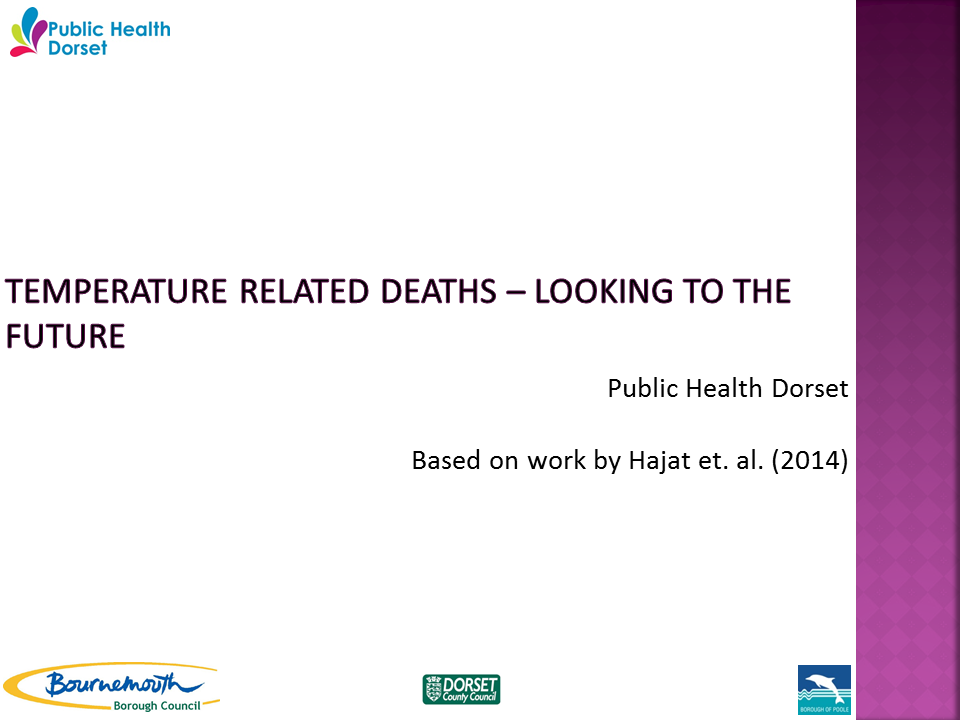
\includegraphics{img/dlSlide1.png}
\caption[Introduction to Temperature Related Death][4.0 cm]{Introduction to temperature related mortality in a future with a warmer climate in West Dorset.}
\end{figure}

\begin{figure}[htbp]
\centering
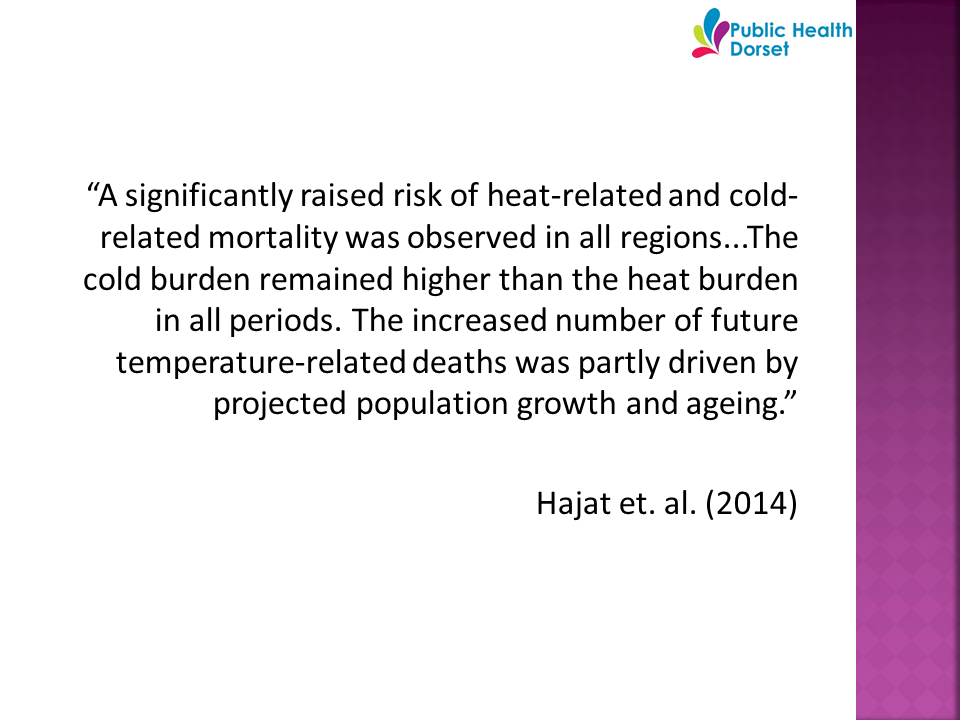
\includegraphics{img/dlSlide2.png}
\caption[Cold not Heat Stress]{Counter intuitive findings were presented up front: we will have more cold related excess mortality that heat related excess mortality in a warmer future West Dorset. Furthermore, the underlying driver of this outcome is the rate of population ageing and growth in West Dorset.}
\end{figure}

\begin{figure}[htbp]
\centering
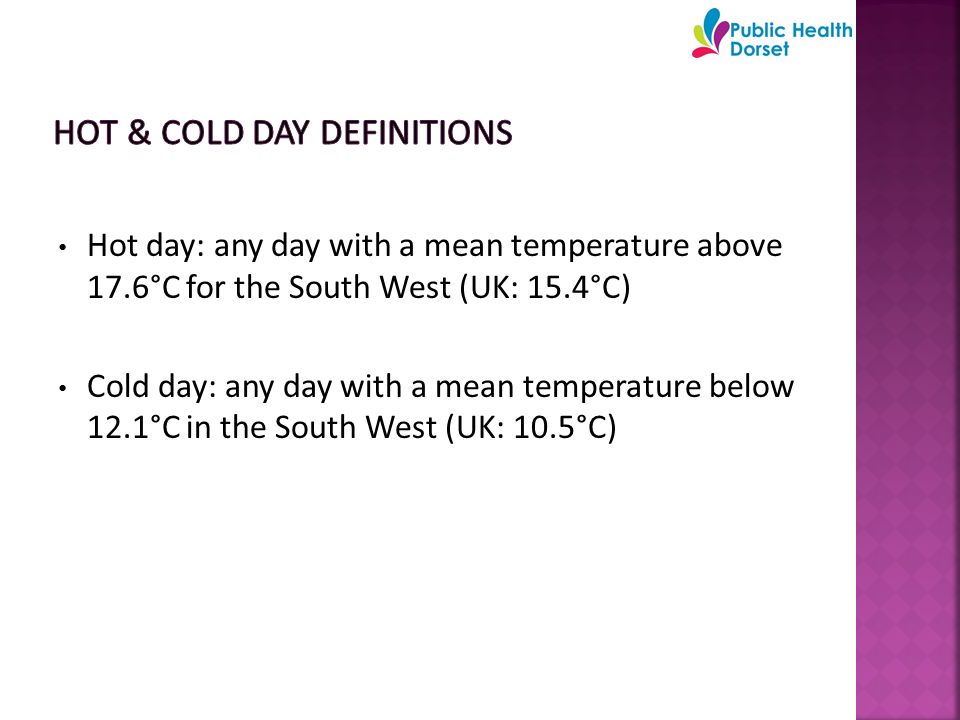
\includegraphics{img/dlSlide3.png}
\caption[Thermal Stress Thresholds are NOT Extreme]{Another counter intuitive find that participants should be aware of is that thermal stress thresholds in West Dorset would be considered quite mild by most people: above 17.6\textdegree C and below 12.1 \textdegree C.}
\end{figure}

\begin{figure}[htbp]
\centering
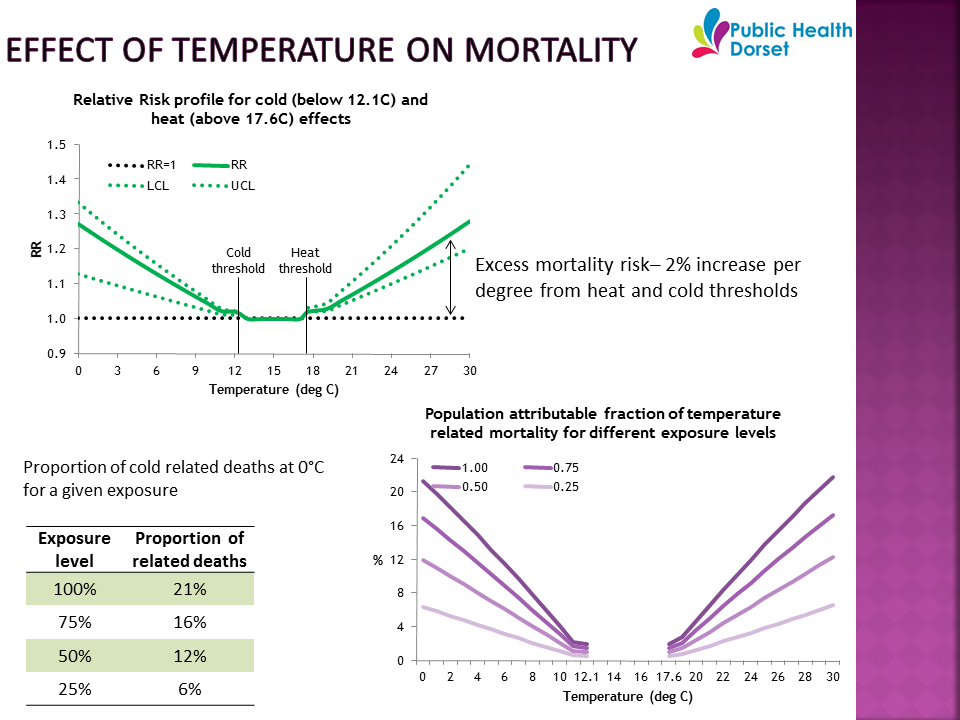
\includegraphics{img/dlSlide4.png}
\caption[Temperature-Mortality Relationship]{The temperature-mortality relationship is statistical in nature and is derived from an examination of mortality and temperature statistics that shows great death rates as one moves above or below the heat and cold, respectively, thresholds. While the causal mechanism is not well articulated and can only surmised at this point, the relationship is nonetheless evident and statistically significant.}
\end{figure}

\begin{figure}[htbp]
\centering
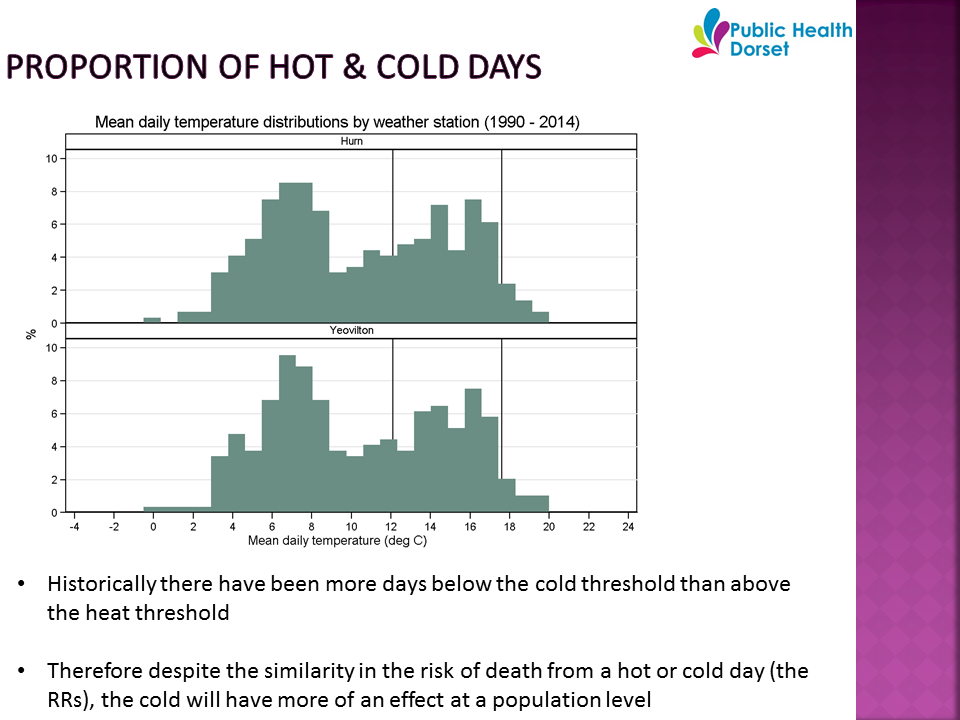
\includegraphics{img/dlSlide5.png}
\caption[Why Cold Stress is Relatively More Important]{Cold stress is going to be responsible for more excess mortality because historically there are more days below the cold threshold than there are days above the heat threshold in West Dorset.}
\end{figure}

\begin{figure}[htbp]
\centering
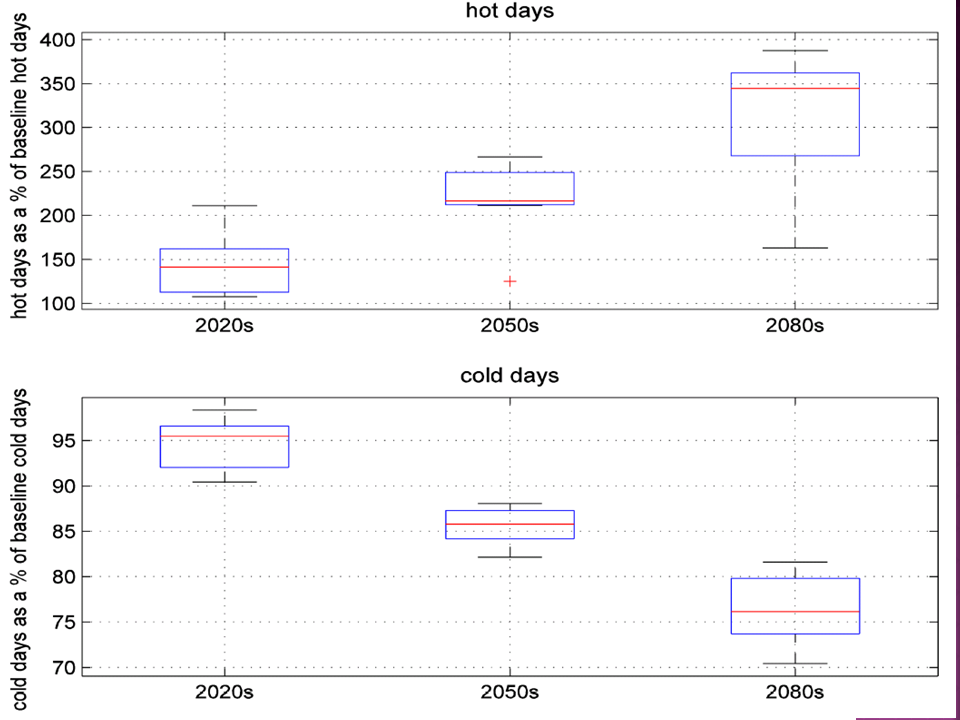
\includegraphics{img/dlSlide6.png}
\caption[Fewer Cold Days More Hot Days]{Although there will be a drop in the number of days below the cold threshold and a rise in the number of days above the heat threshold this change is not likely to be enough by 2030s to make heat excess mortality more important than cold excess mortality.}
\end{figure}

\begin{figure}[htbp]
\centering
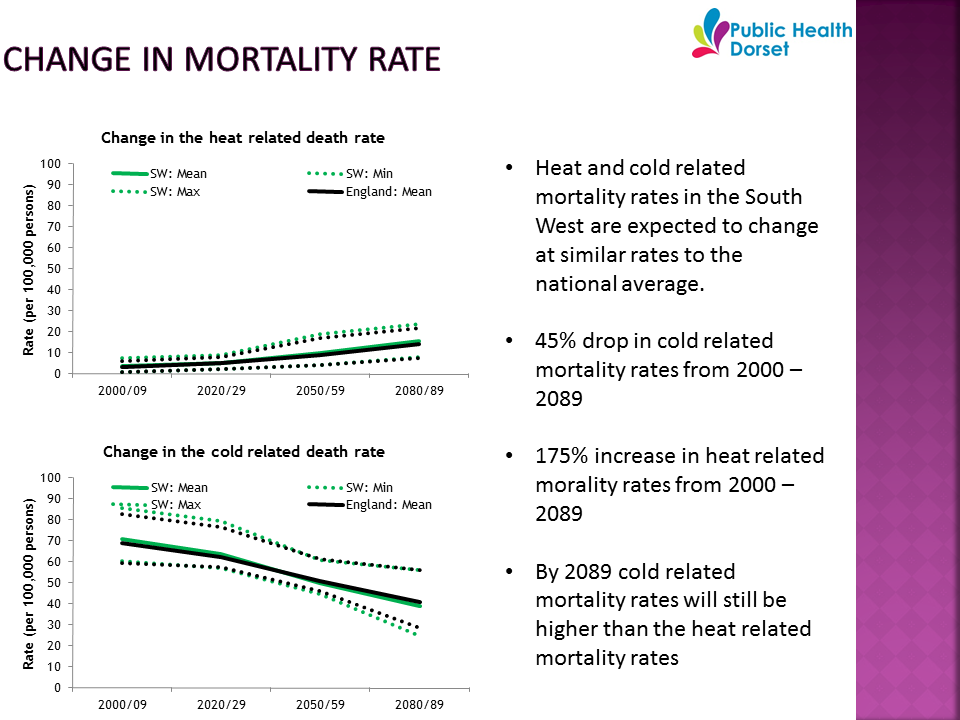
\includegraphics{img/dlSlide7.png}
\caption[Change in Mortality Rate]{The expected changes in mortality, down for cold related mortality and up for heat related mortality, are consistent with that calculated for all of England.}
\end{figure}

\begin{figure}[htbp]
\centering
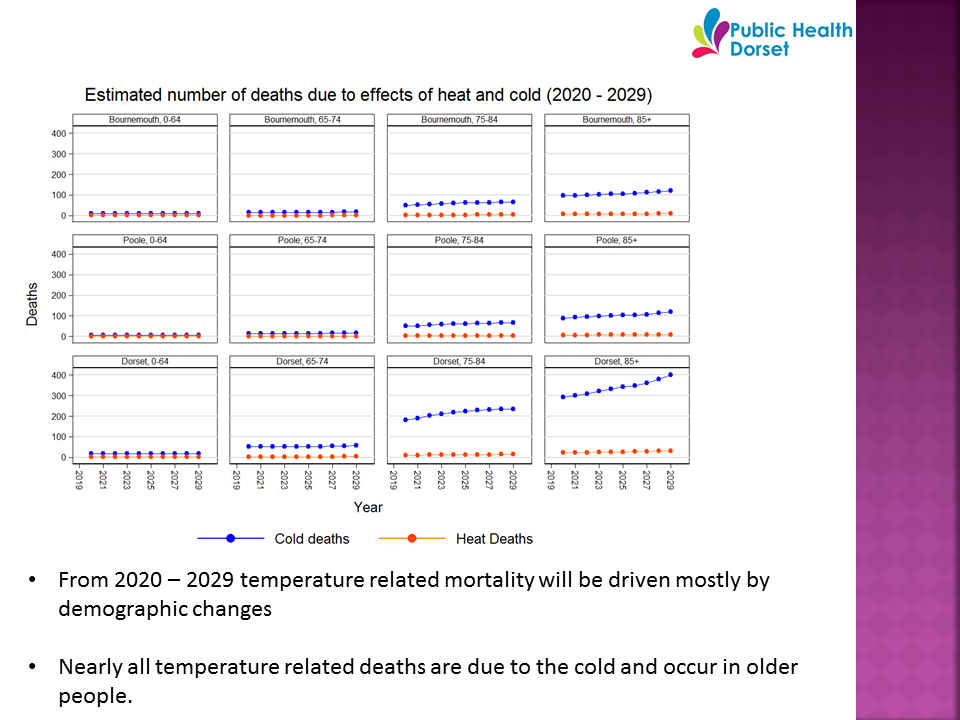
\includegraphics{img/dlSlide8.png}
\caption[Estimated Number of Deaths]{In a comparison of Bournemouth, Poole and Dorchester, the most noticeable difference is that Dorchester's inland setting means that there are more days in which the cold threshold is exceeded. The similarity amongst locations is that the cold related deaths always exceed heat related deaths and that the rathe of change over time is consistent.}
\end{figure}

\begin{figure}[htbp]
\centering
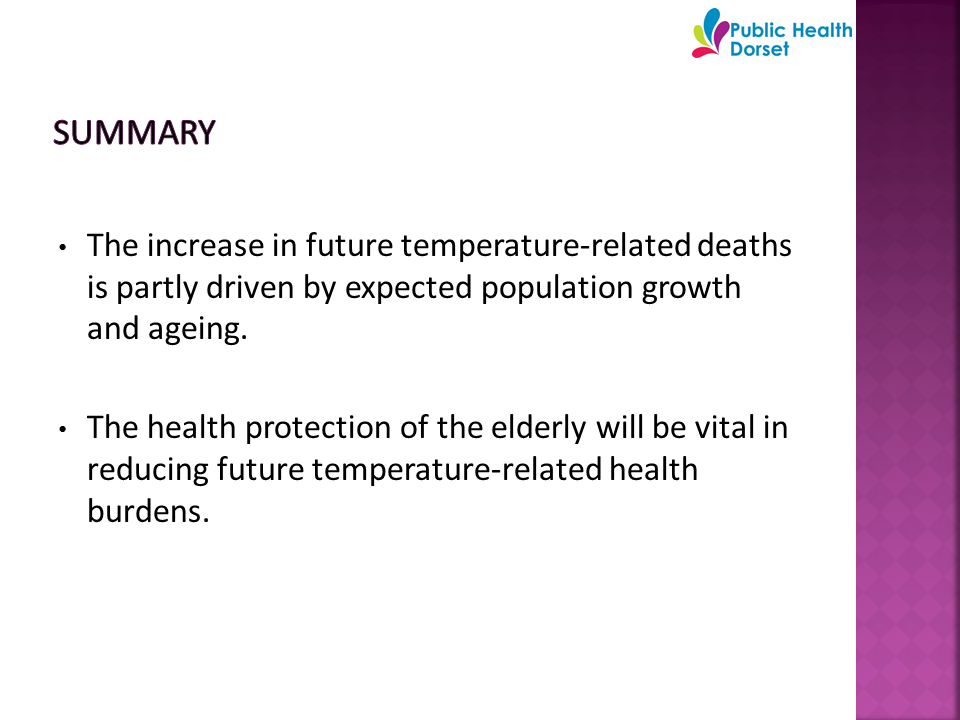
\includegraphics{img/dlSlide9.png}
\caption[Summary]{In summary, participants are reminded that the ageing and population growth trends are driving this future problem - we can't change this. We need to focus on mitigating impacts of both heat and cold stress amongst the large elderly population of a West Dorset in 2030.}
\end{figure}

\begin{figure}[htbp]
\centering
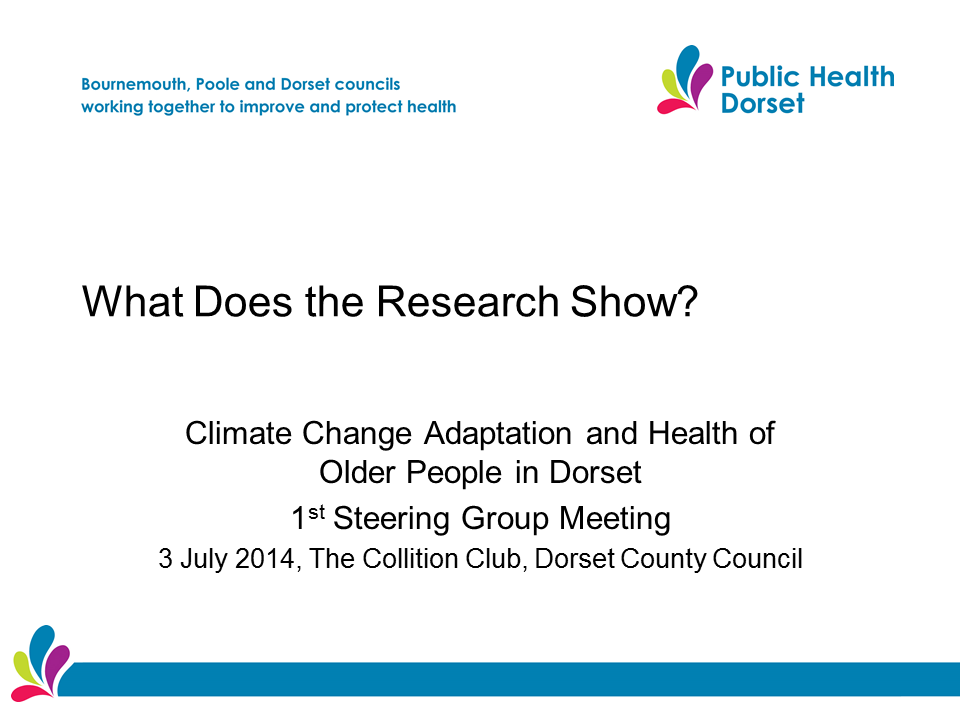
\includegraphics{img/wrsSlide1.png}
\caption[Introduction to Project]{Introducing the steering group to what the current relevant research shows.}
\end{figure}

\begin{figure}[htbp]
\centering
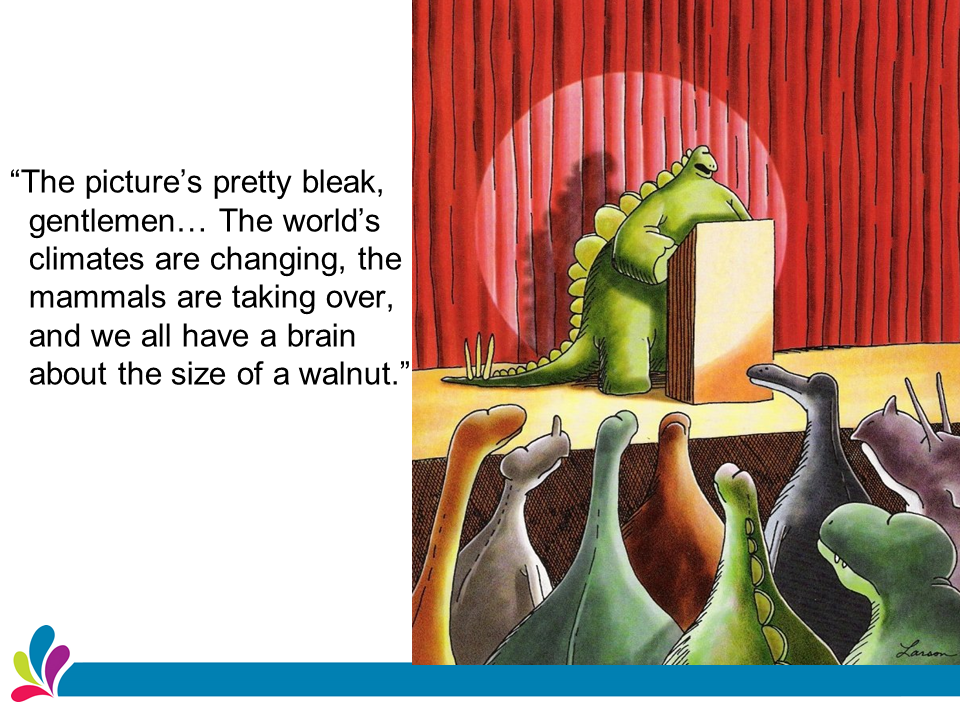
\includegraphics{img/wrsSlide2.png}
\caption[Project Challenge]{We identified early, the complexity of the topic this project seeks to explore. Additionally, the key challenge ahead in this project, would be to get the attention of colleagues and other key stakeholders, because this is a `future' problem and not of immediate concern to most.}
\end{figure}

\begin{figure}[htbp]
\centering
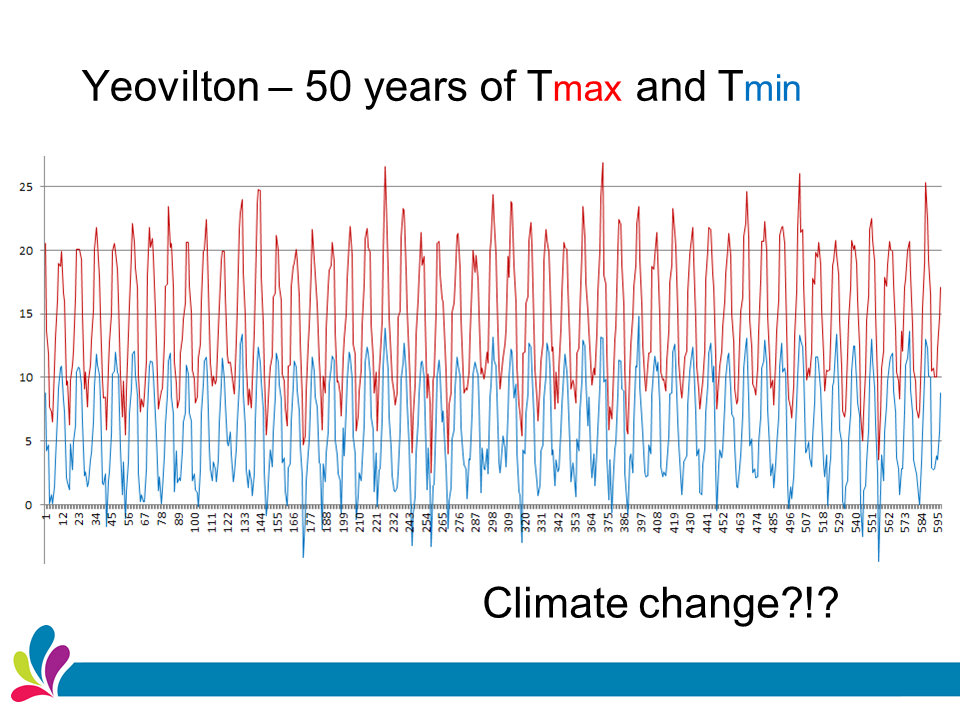
\includegraphics{img/wrsSlide3.png}
\caption[Climate Change Complexity]{We noted that understanding climate change involved understanding the role of the past and present climate in population health. It's not obvious to everyone. What should stakeholders make of these local minimum and maximum temperature curves from Yeovilton.}
\end{figure}

\begin{figure}[htbp]
\centering
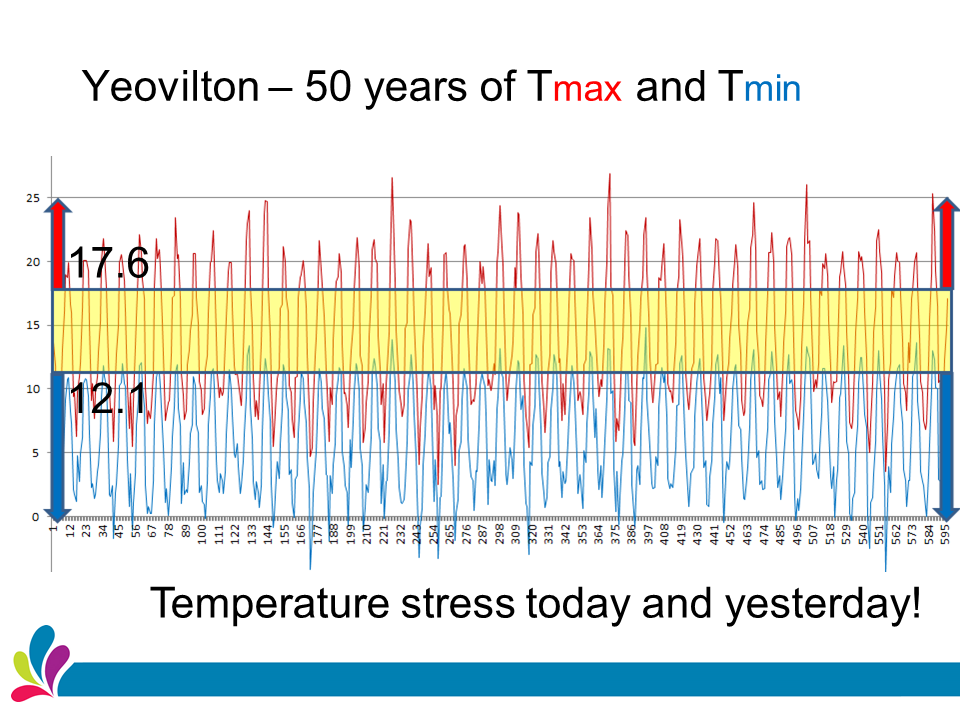
\includegraphics{img/wrsSlide4.png}
\caption[Project Thermal Stress Focus]{However, the key foci of the project can be made more clear, and the complexity brought in focus if we can visually direct stakeholder attention to the temperature thresholds that do impact on human health. We can use this relationship to explore future impacts on health, or at least one dimension of future impact.}
\end{figure}

\begin{figure}[htbp]
\centering
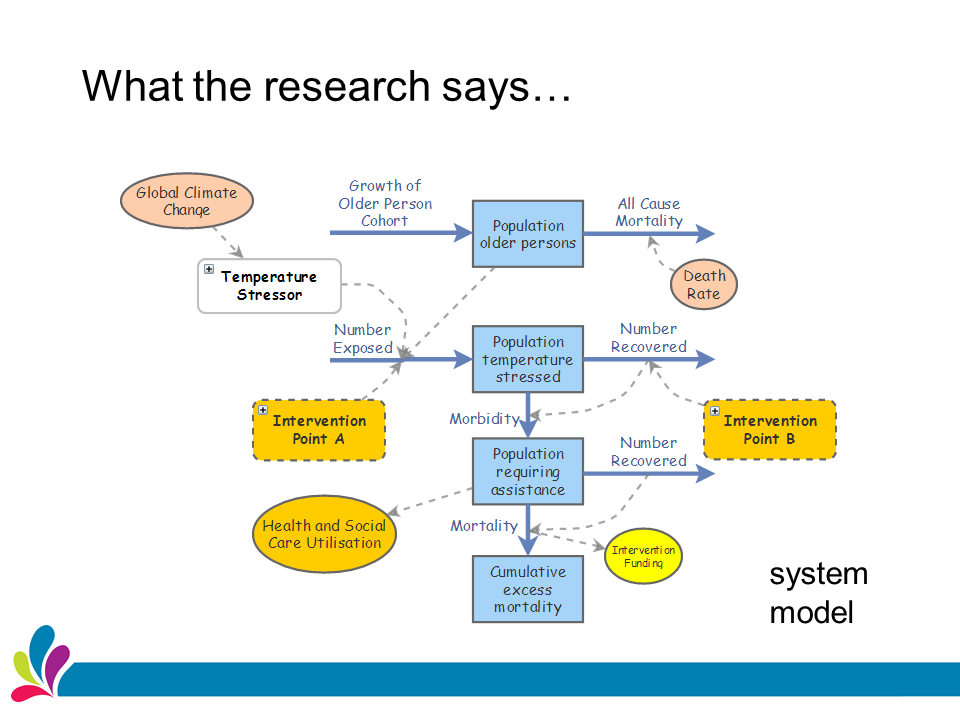
\includegraphics{img/wrsSlide5.png}
\caption[Communicating with a Systems Model]{An initial systems model created on-line using \emph{Insight Maker} captures what we believe to be the essence of problem involving the primary impact of climate change on older people in Dorset.}
\end{figure}

\begin{figure}[htbp]
\centering
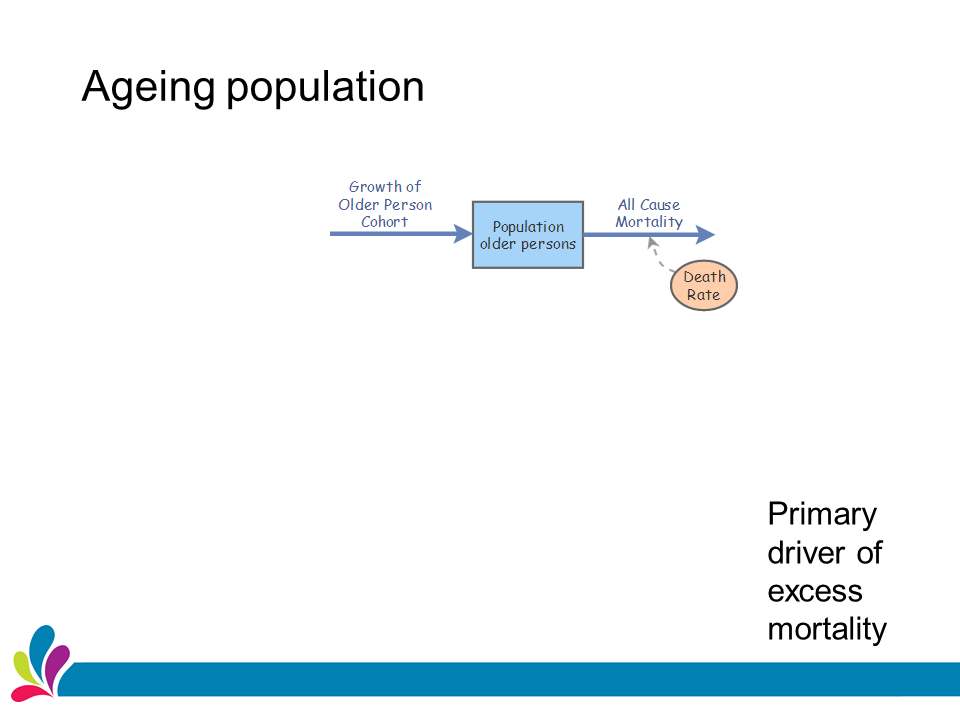
\includegraphics{img/wrsSlide6.png}
\caption[Primary Driver of Excess Mortality]{It is not intuitively obvious that the primary driver of excess mortality in 30 years time, in respect of climate impact on older people, will be our ageing population. Nonetheless, this is a key component and there is not much that can be done about it.}
\end{figure}

\begin{figure}[htbp]
\centering
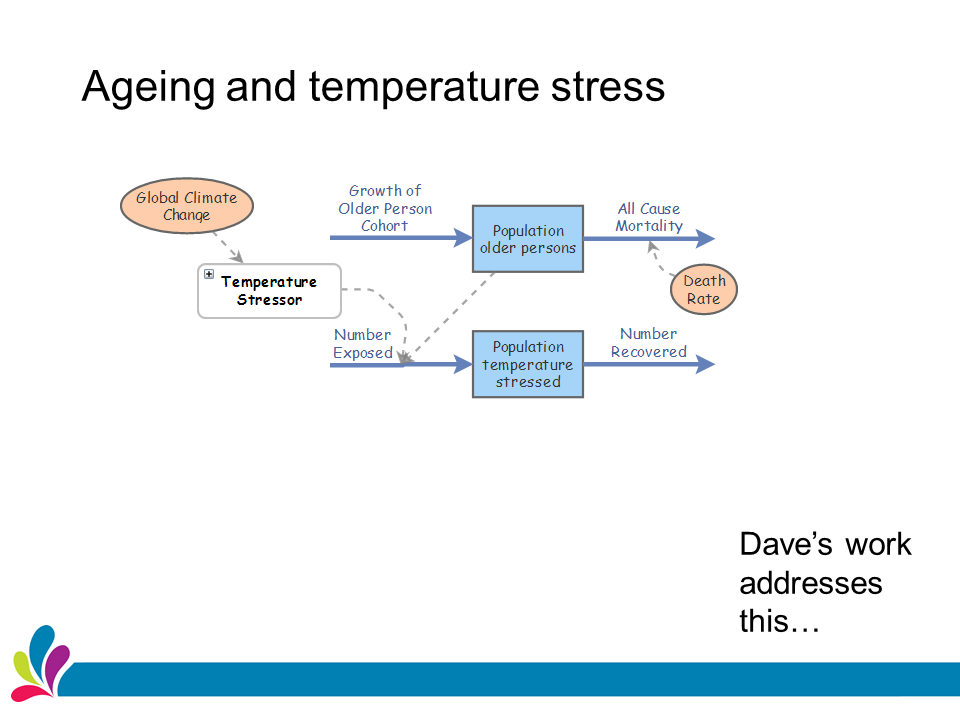
\includegraphics{img/wrsSlide7.png}
\caption[Ageing and Thermal Stress]{The `ageing' driver provides a growing population of people who will be disproportionately affected by thermal stress.}
\end{figure}

\begin{figure}[htbp]
\centering
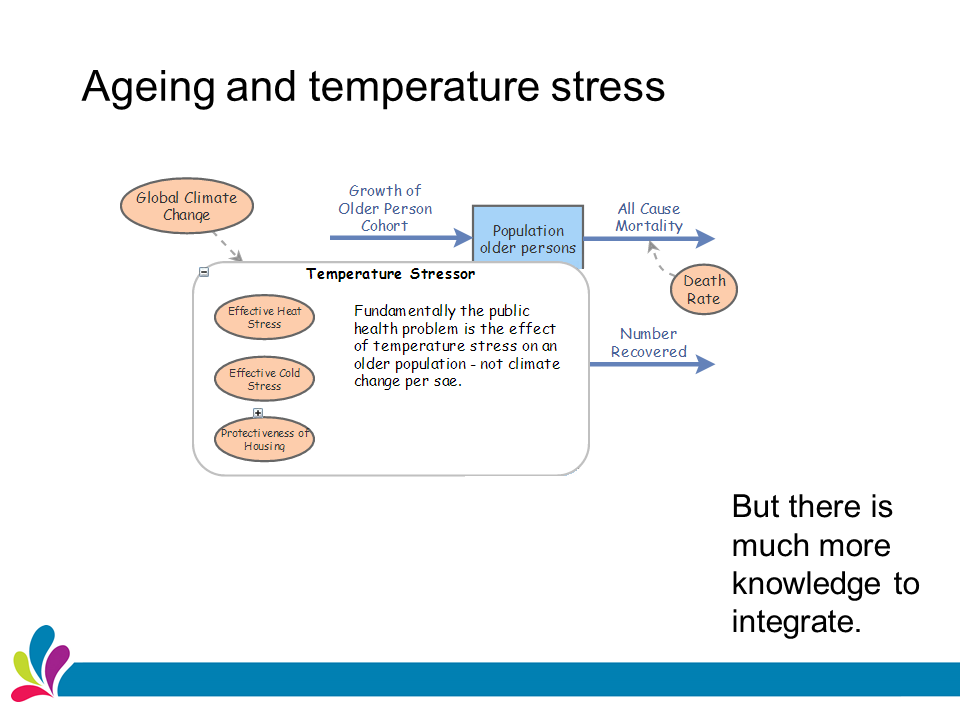
\includegraphics{img/wrsSlide8.png}
\caption[Unpacking Complexity Thermal Stress]{Using Insight Maker, participants will be able to unpack in a structured way different levels of knowledge -- in this case we could further unpack thermal stress into heat and cold stresses. Furthermore, we might chose to include the protective role of housing in this project [note that we were not able to include housing effect in this project].}
\end{figure}

\begin{figure}[htbp]
\centering
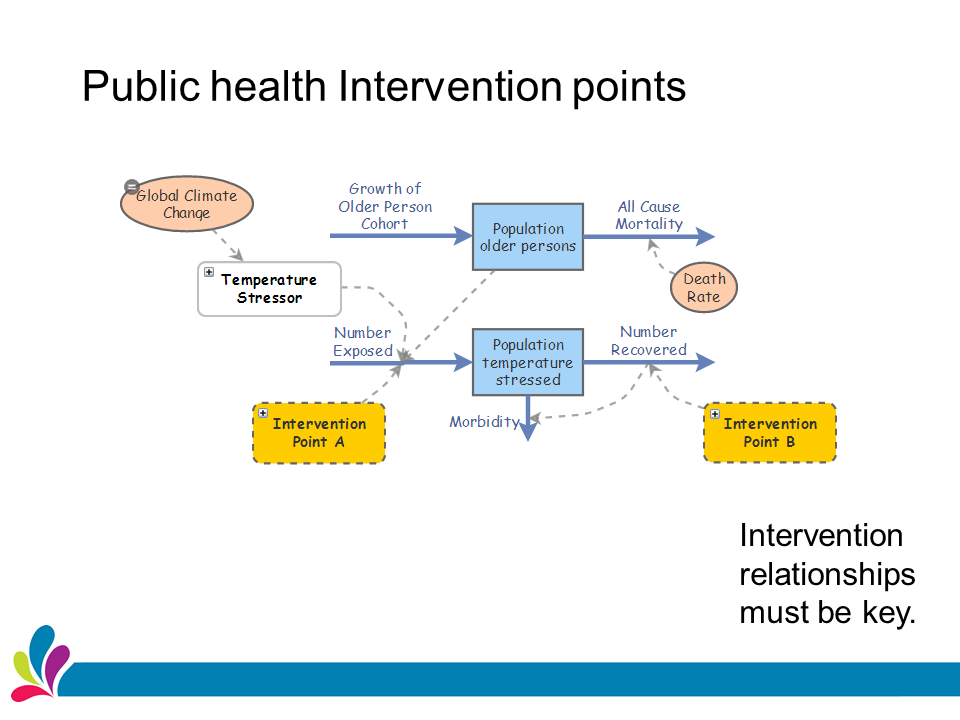
\includegraphics{img/wrsSlide9.png}
\caption[Visualising Public Health Interventions]{We can use this Systems Model to develop a shared understanding of where it might be possible to implement public health interventions.}
\end{figure}

\begin{figure}[htbp]
\centering
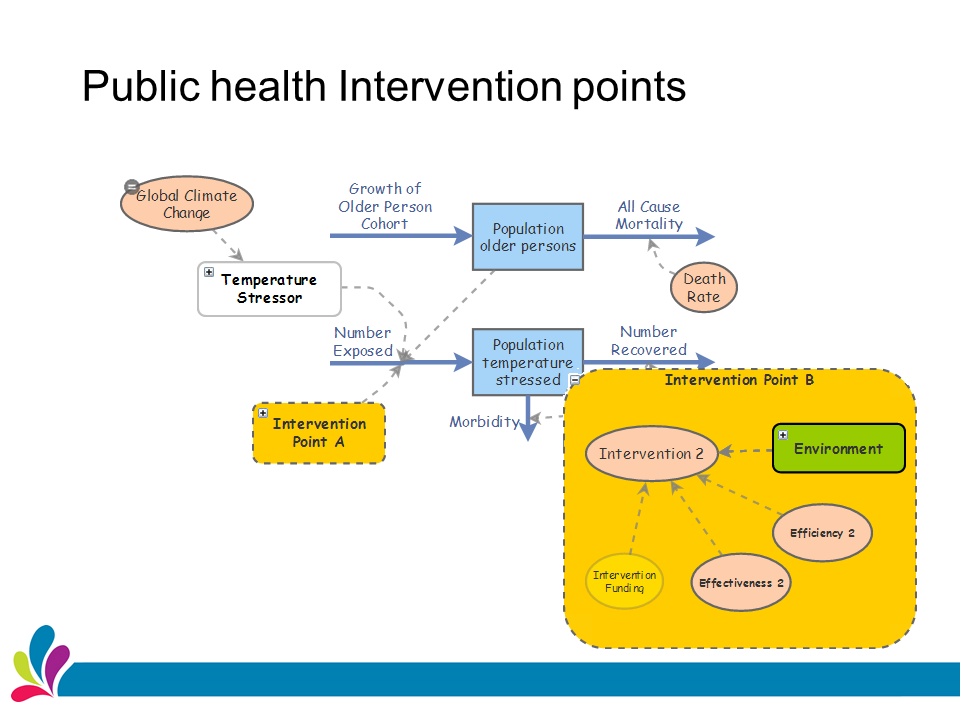
\includegraphics{img/wrsSlide10.png}
\caption[Unpacking Public Health Interventions]{Using Insight Maker, participants will be able to unpack the components of a public health intervention. Note that we did develop this aspect of the model further during the project.}
\end{figure}

\begin{figure}[htbp]
\centering
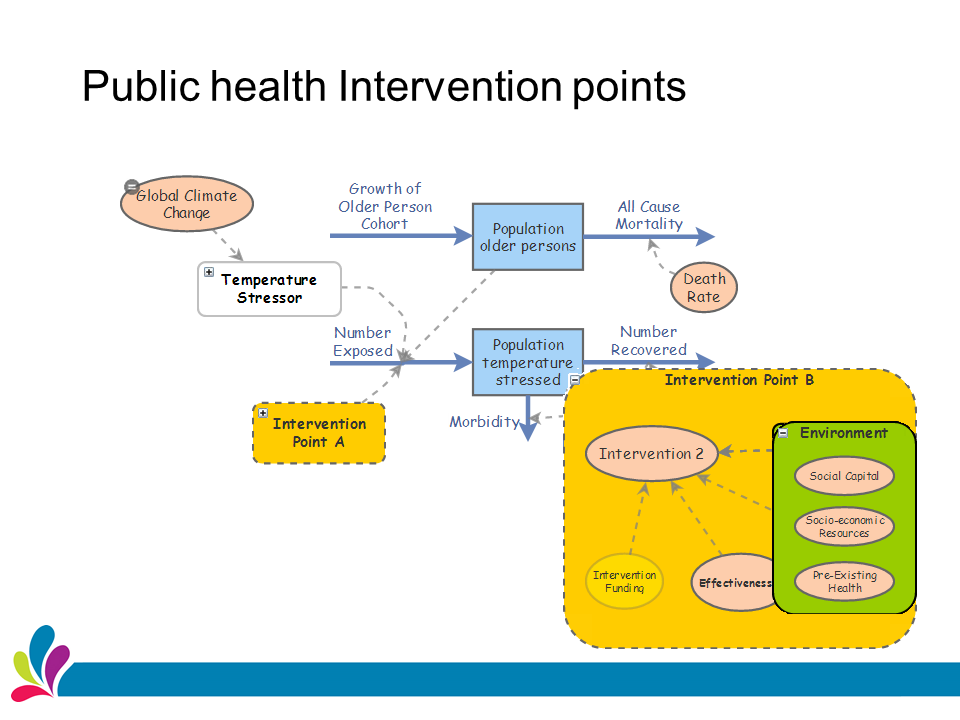
\includegraphics{img/wrsSlide11.png}
\caption[Unpacking Interventions Even Further]{With the development of Systems Models in Insight Maker, one can develop multiple levels of detail, which participants can explore depending on what they are most interested in. Importantly, the model can be used at a very high level, which `hides' detail not required by some participants.}
\end{figure}

\begin{figure}[htbp]
\centering
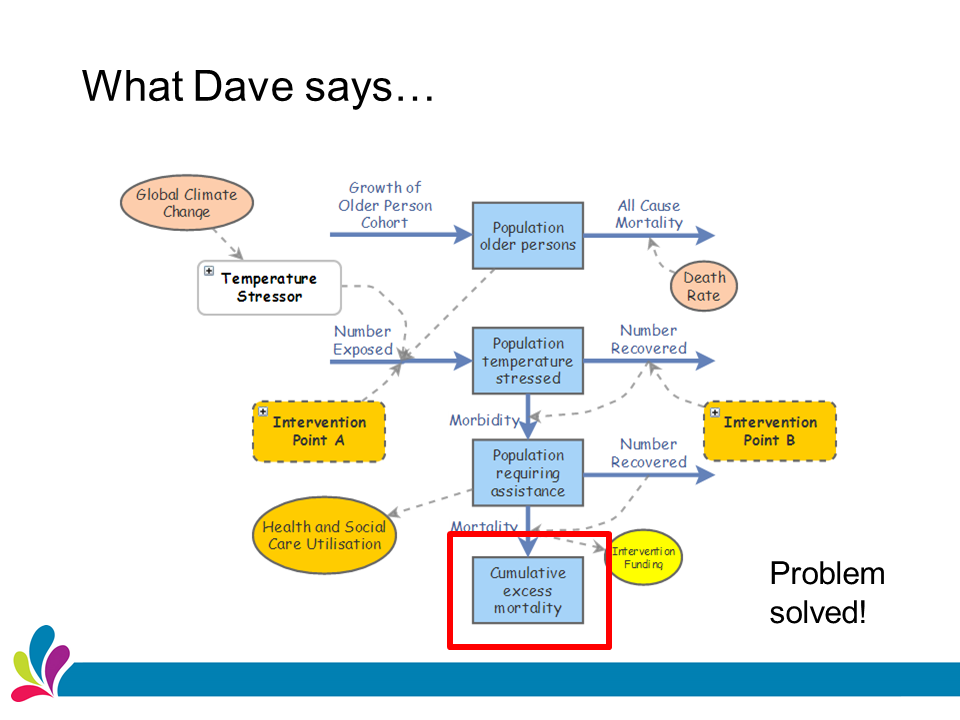
\includegraphics{img/wrsSlide12.png}
\caption[Simulating Excess Mortality]{The Systems Model explicitly and visually represented the quantities that are being simulated. In this version of the model, impact is being `indicated' by the measure of `Cumulative Excess Mortality'.}
\end{figure}

\begin{figure}[htbp]
\centering
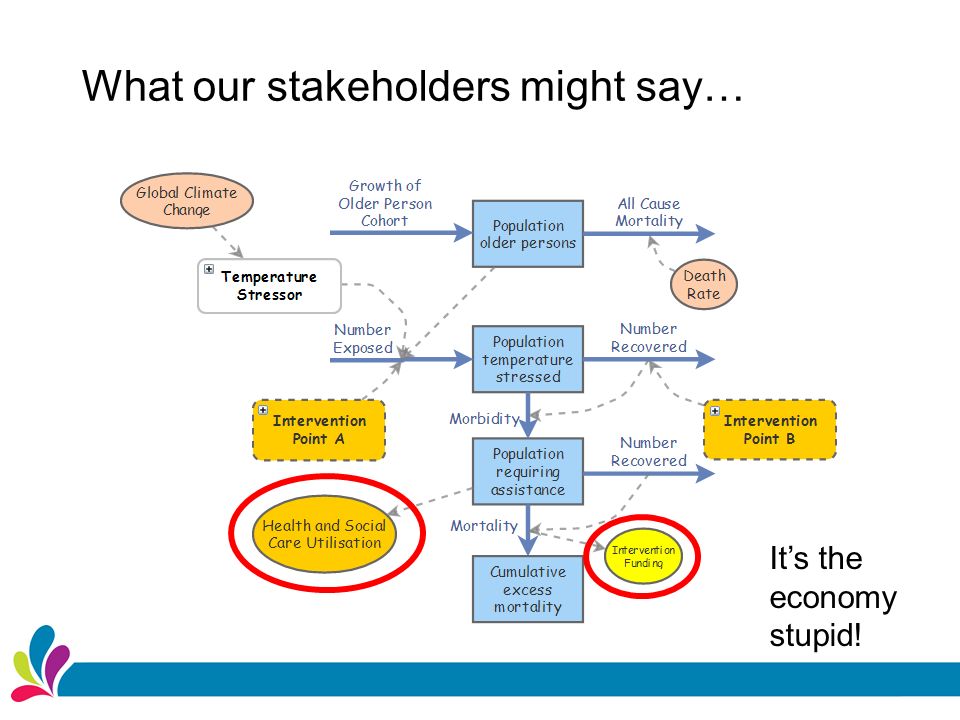
\includegraphics{img/wrsSlide13.png}
\caption[Extending the Systems Model]{This systems model can be extended to look at other 'indicators' of climate change impact due to thermal stress on older people and one could examine the potential impact on intervention funding of large or unexpected increases in excess mortality.}
\end{figure}

\begin{figure}[htbp]
\centering
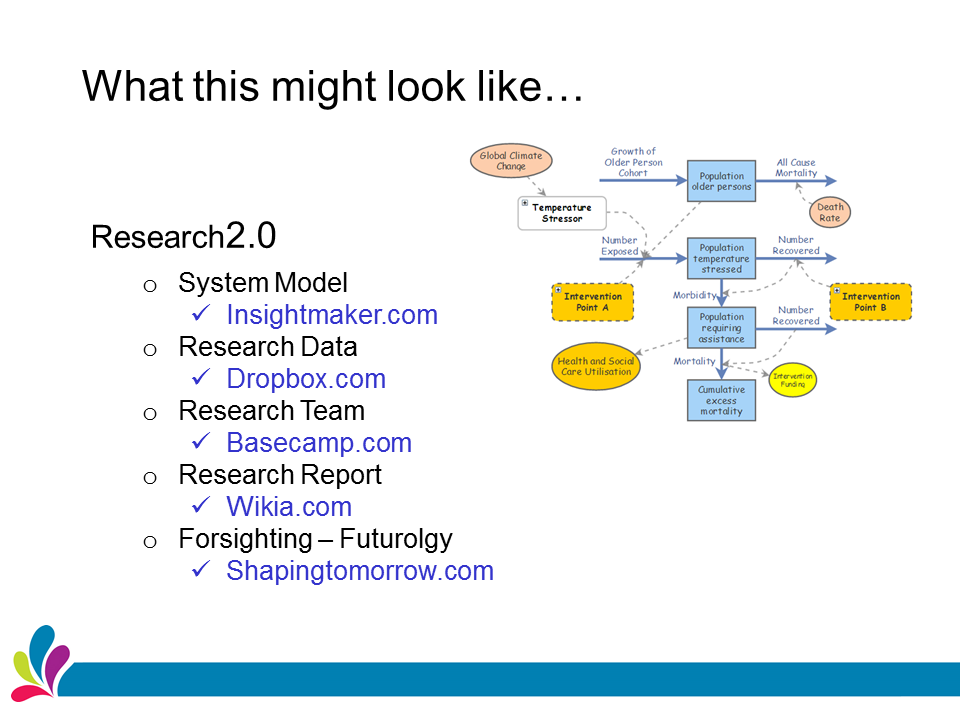
\includegraphics{img/wrsSlide14.png}
\caption[Collaborative Research2.0]{The necessity of collaborating on projects at distance means that we need to consider using on-line tools, where we might otherwise look to more traditional desktop software packages.}
\end{figure}

\begin{figure}[htbp]
\centering
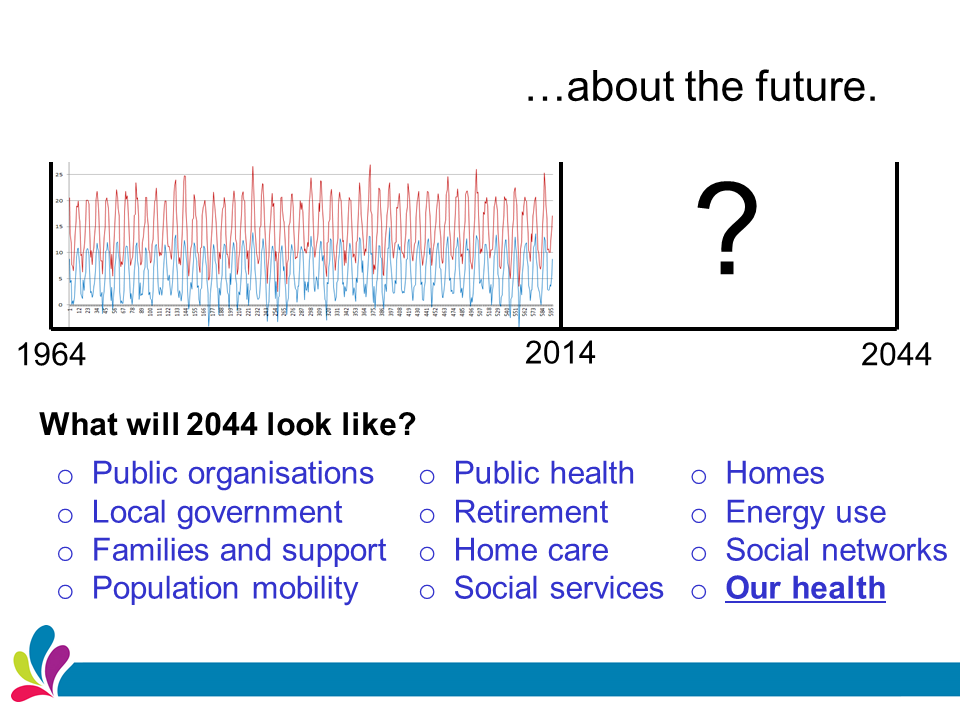
\includegraphics{img/wrsSlide15.png}
\caption[The Role of Futures Studies]{The role of futures studies needs to be considered in the context of this project, because `climate change' isn't the only `change' we are likely to experience, therefore simulating `impacts' in 30 years time, requires a more comprehensive look at impacts.}
\end{figure}

\begin{figure}[htbp]
\centering
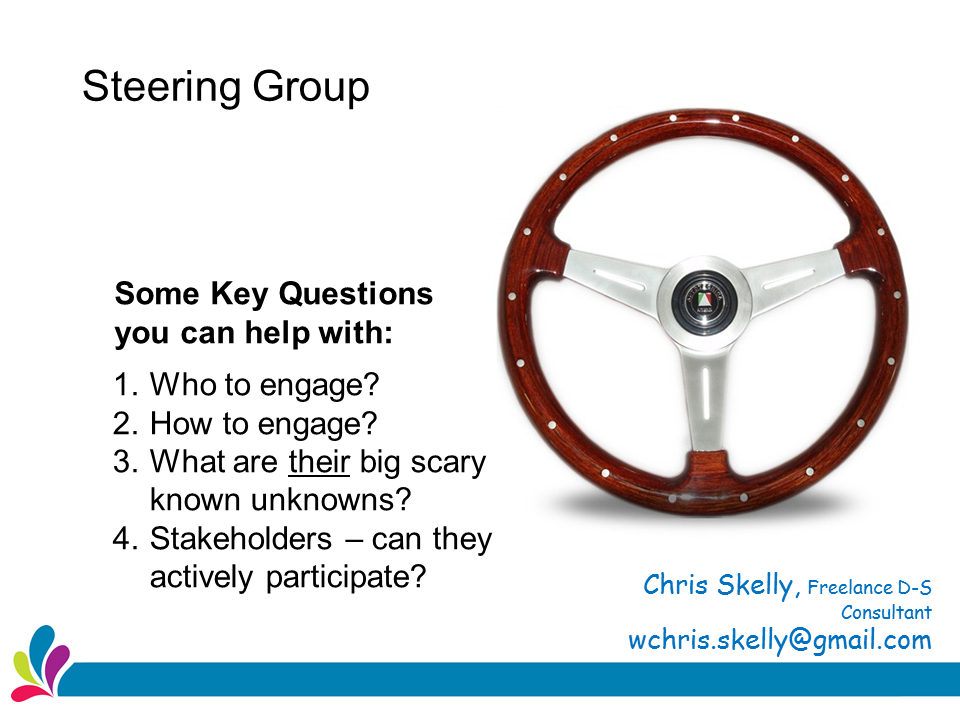
\includegraphics{img/wrsSlide16.png}
\caption[Steering Group Rationale]{We started this project hoping to set up a steering group that would enhance our engagement with stakeholders and provide some direction to the research we were undertaking. Note that we were unsuccessful in actively engaging a steering group in this regard.}
\end{figure}

